
%%%%%%%%%%%%%%%%%%%%%%%%%%%%%%%%%%%%%%%%%%%%%%%%%%%%%%%%%%%%%%%%%%%%%%%%%%%%%
%%%%% Basic C++ %%%%%%%%%%%%%%%%%%%%%%%%%%%%%%%%%%%%%%%%%%%%%%%%%%%%%%%%%%%%%
%%%%%%%%%%%%%%%%%%%%%%%%%%%%%%%%%%%%%%%%%%%%%%%%%%%%%%%%%%%%%%%%%%%%%%%%%%%%%
\begin{frame}
\pointedsl{
	Basics
}
\end{frame}

% TODO
% Content:
% 1. Variables (declaration, assignment, operations)
% 2. Types (list: char, short, int, float, double, bool, void; typedef)
% 3. Expressions (unary, binary, arithmetic, comparator, bitwise)
% 4. Conditions (if, else if, else)
% 5. Loops (for, while, do while)
% 6. Functions (declaration, definition, signature /!\ types -> diff fun)
% 7. Arrays

%%%%%%%%%%%%%%%%%%%%%%%%%%%%%%%%%%%%%%%%%%%%%%%%%%%%%%%%%%%%%%%%%%%%%%%%%%%%%
\lstset{numbers=none}
\begin{frame}[fragile]
\frametitle{Variables}
\begin{lstlisting}
int x; // declare a variable of type "int"
x = 7; // assign a value to "x"
int y = 2; // declare and assign 2 to "y"
y = y * 2; // multiply by 2, then reassign
y *= 2; // shorter version of above
int z = (y - 2) * x; // z equals 42
\end{lstlisting}
\misc{
	\textbf{Variables} are used to store data.
	
	Each variable posesses 
	\begin{itemize}
		\item a \emph{name} (\ctext{x}, \ctext{y}, \ctext{z})
		\item a \emph{type} (\ctext{int} for integer)
	\end{itemize}
	that enable the program to locate and interpret the data.
}
\end{frame}

%%%%%%%%%%%%%%%%%%%%%%%%%%%%%%%%%%%%%%%%%%%%%%%%%%%%%%%%%%%%%%%%%%%%%%%%%%%%%
\begin{frame}[fragile]
\frametitle{Variable types}
\begin{center}
\includegraphics[width=0.6\textwidth]{figures/bits_black}
\end{center}
\misc{
	Computer data consists of sequences of '0' and '1' (bits).
	
	The type of a variable provides an interpretation of the data sequence. Without a type, the bits may mean anything.
}
\end{frame}

\begin{frame}[fragile]
\frametitle{Variable types}
\misc{
	Fundamental types include:
	\begin{itemize}
		\item \textbf{Integer types}: \ctext{char}${}^{(*)}$, \ctext{short}, \ctext{int}, \ctext{long} (each \ctext{signed} or \ctext{unsigned})
		\item \textbf{Floating point types}: \ctext{float}, \ctext{double}
		\item \textbf{Boolean type:} \ctext{bool}
	\end{itemize}
	Each has a specific \emph{size} in memory and can only represent a limited amount of distinct values (the type \emph{range}).
}
\begin{lstlisting}
unsigned int n = 1; bool f = true;
char c = 'a'; double pi = 3.14159;
\end{lstlisting}
\end{frame}

\begin{frame}[fragile]
\frametitle{Variable types}
\begin{center}
\includegraphics[width=0.6\textwidth]{figures/bits}
\end{center}
\begin{lstlisting}
int i = 1;
char c = '1';
float f = 1.0f;
\end{lstlisting}
\end{frame}

%%%%%%%%%%%%%%%%%%%%%%%%%%%%%%%%%%%%%%%%%%%%%%%%%%%%%%%%%%%%%%%%%%%%%%%%%%%%%
\lstset{language=C++,numbers=none}
\begin{frame}[fragile]
\frametitle{Declaration and definition}
\begin{lstlisting}
void process(int x); // declare a function
int x; // declare a variable
x = 10; // assign a value
process(x);
// declaration and definition
int sum(int a, int b){ return a + b; }
// declaration and assignment
int y = sum(x, 2);
\end{lstlisting}
\misc{
	Every variable, type or function must be declared before being used. They can then be defined anywhere.
	
	\textbf{Note}: variables automatically receive a default value corresponding to $0$.
}
\end{frame}

%%%%%%%%%%%%%%%%%%%%%%%%%%%%%%%%%%%%%%%%%%%%%%%%%%%%%%%%%%%%%%%%%%%%%%%%%%%%%
\begin{frame}[fragile]
\frametitle{Flow control}
\begin{center}
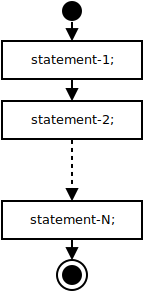
\includegraphics[width=0.7\textwidth]{figures/flow}
\end{center}
\misc{
	The usual conditional blocks are available
	\begin{itemize}
		\item \ctext{if}, \ctext{else if}, \ctext{else} and \ctext{switch}
	\end{itemize}
	as well as loop structures
	\begin{itemize}
		\item \ctext{for}, \ctext{while} and \ctext{do while}
	\end{itemize}
}
\end{frame}

%%%%%%%%%%%%%%%%%%%%%%%%%%%%%%%%%%%%%%%%%%%%%%%%%%%%%%%%%%%%%%%%%%%%%%%%%%%%%
\begin{frame}[fragile]
\frametitle{Arrays}
\begin{columns}[c]
  \begin{column}{0.5\textwidth}
\lstset{language=C++,numbers=left}
\begin{lstlisting}
int a[3] = { 1, 0 };
a[1] = 42;
// a[2] == 0
\end{lstlisting}
  \end{column}
  \begin{column}{0.5\textwidth}
    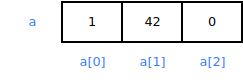
\includegraphics[width=0.95\textwidth]{figures/array0}
  \end{column}
\end{columns}
\misc{
	\emph{Arrays} are continuous blocks of memory that store multiple elements of a same type. They use $0$-based indexing.
}
\end{frame}
